\documentclass[10pt]{article}
\usepackage[utf8]{inputenc}
\usepackage[T1]{fontenc}
\usepackage{amsmath}
\usepackage{amsfonts}
\usepackage{amssymb}
\usepackage[version=4]{mhchem}
\usepackage{stmaryrd}
\usepackage[margin=0.5in]{geometry}
\usepackage{graphicx}
\begin{document}

\noindent

\textbf{IMPORTANT: This proof was automatically translated from original in Czech language to English!}

\vskip 0.5cm

(0.5 point) Decide whether the following language $L_1$ is regular or not. If the language is not regular, formally prove this claim. If the language is regular, describe it using one of the formalisms for describing regular languages (i.e., FA (Finite Automaton), RG (Regular Grammar), or RE (Regular Expression)). Also, find the smallest pumping lemma constant $p$ (whose existence is guaranteed by the pumping lemma for regular languages) and explain why your constant is correct and minimal.

$$L_1=\left\{w: w \in\{\mathtt{a}, \mathtt{b}\}^{*} \wedge|w|_{\mathrm{a}} \bmod 3=|w|_{\mathrm{b}}\right\} \cap\left\{\mathtt{a}^{m} \mathtt{b}^{j} \mathtt{b}^{i}: m, j, i \in \mathbb{N}_{0} \wedge j<m\right\}$$

\noindent
Note: Using the notation $|x|_a$ to denote the number of symbols $a$ in the string $x$.

\section*{Solution:}

\begin{description}
\item[(1)]

The language $L_1$ is the intersection of two languages $L_{l}$ and $L_{r}$ (with $l$ as "left", $r$ as "right"), i.e., $L_1 = L_l \cap L_r$. Let's examine the individual languages $L_l$ and $L_r$:

Language $L_l$:

$$L_l = \left\{w: w \in\{\mathtt{a}, \mathtt{b}\}^{*} \wedge|w|_{\mathrm{a}} \bmod 3=|w|_{\mathrm{b}}\right\}$$

$L_l$ represents all possible strings over the alphabet $\Sigma = \left\{a, b\right\}$, where the number of symbols $b$ is equal to the number of symbols $a$ modulo 3. As a consequence, the number of symbols $b$ is at least $0$ and at most $2$. Examples of possible strings from this language:

$$L_l = \left\{
\epsilon,
ab, ba, aabb, abab, bbaa, baab, aaa, aaaab, aabaa, aaaaabb, aaaaaa, \dots 
\right\}$$

Language $L_r$:

$$L_r = \left\{\mathtt{a}^{m} \mathtt{b}^{j} \mathtt{b}^{i}: m, j, i \in \mathbb{N}_{0} \wedge j<m\right\}$$

Examples of strings:

$$L_r = \left\{
a, ab, abb, abbb, abbbb, \dots, aab, aabb, aabbb, aaabbbb, \dots 
\right\}$$

We notice that $L_r$ specifies a certain structure of the string—all symbols $a$ occur only on the left, and symbols $b$ only on the right. 

Furthermore, we see that the minimal string is $w = a$, because we have the condition $j < m$, and we also know that the smallest possible $j$ is $0$ (since $j \in \mathbb{N}_{0}$), which means that $m$ cannot be $0$ (otherwise, we would have a contradiction that $j$ must be less than zero and at the same time greater than or equal to zero). That is, essentially, $m \geq 1$, i.e., $m \in \mathbb{N}$ but excluding zero.

Another observation is that $i$ can be arbitrary and does not depend on any other variable. That is, for all $m \in \mathbb{N}$, if we fix $j = 0$, then using $i$ we can generate any number of symbols $b$, and it will always hold that $j < m$.

If we combine both observations above, we can simplify the language $L_r$ as follows:

$$L_r = \{\mathtt{a}^{m} \mathtt{b}^{j} \mathtt{b}^{i}: m, j, i \in \mathbb{N}_{0} \wedge j<m\}
= \{\mathtt{a}^{m} \mathtt{b}^{i}: i \in \mathbb{N}_{0} \land m \in \mathbb{N}\}$$

In summary, we obtain the simplified intersection of the languages:

$$L_1=\left\{w: w \in\{\mathtt{a}, \mathtt{b}\}^{*} \wedge|w|_{\mathrm{a}} \bmod 3=|w|_{\mathrm{b}}\right\} \cap \left\{\mathtt{a}^{m} \mathtt{b}^{i}: i \in \mathbb{N}_{0} \land m \in \mathbb{N}\right\}$$

We notice that $L_r$ gives us the structure of the language $L_1$—that is, on the left are always symbols $a$, and on the right are always symbols $b$. The next and last restriction that $L_r$ makes is that the minimal string is $a$. Otherwise, it can contain any number of additional symbols $a$ on the left and any number of symbols $b$ on the right.

If we now apply the restriction from $L_l$ to $L_r$, we see that on the right, we can have $0$, $1$, or $2$ symbols $b$ (depending on the number of symbols $a$ on the left).

We can therefore simplify the language $L_1$ as:

$$L_1 = \left\{
\mathrm{a}^{m}\mathrm{b}^{n}: m \in \mathbb{N}, n \in \mathbb{N}_{0} \land |w|_{\mathrm{a}} \bmod 3 = |w|_{\mathrm{b}}
\right\}$$

To prove that this language is regular, we could utilize closure properties for intersection. That is, if we could prove that $L_l$ and $L_r$ are regular, then their intersection would also be regular. But now that we have the simplified description $L_1$, which is equivalent, it will be much easier to prove the regularity of this simplified description—that is, we need to describe it using one of the formalisms for regular languages. And we will do that using this finite automaton:

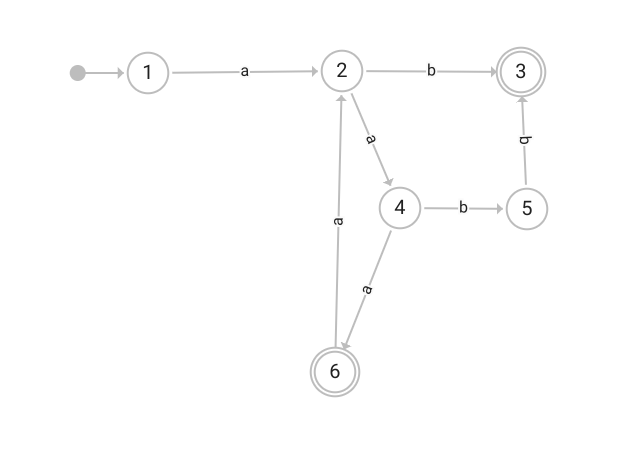
\includegraphics[width=\textwidth]{automat.png}

That is, there exists a FA (in this case, a DFA) generating this language; therefore, this language is regular. 

\item[(2)]

Formally, we will verify whether this language has the pumping property (we already know that it should have it; otherwise, this language could not be regular).

We want to verify that there exists a constant $p \in \mathbb{N}$ such that for every string $w \in L_1$, where if $|w| \geq p$, then there exists some decomposition of the string $w = xyz$ such that $|y| \geq 1$ and also $|xy| \leq p$ and also $\forall k \in \mathbb{N}_{0}$ it holds that $xy^{k}z \in L_1$.

Formally:

$$(\exists p \geq 1)(\forall w \in L_1)[|w| \geq p \Rightarrow (\exists x, y, z \in \Sigma^{*})(w = xyz \land |xy| \leq p \land |y| \geq 1 \land (\forall k \geq 0)(xy^{k}z \in L_1))] $$

At the same time, we need to find this constant $p$ minimal.

Let's try $p = 1$:

Take the string $w = a$, then there exists exactly one decomposition $w$: 

\begin{align*}
& x = \epsilon \\
& y = a \\
& z = \epsilon \\
\end{align*}

Then for $k = 0$, we get $xy^{0}z = \epsilon a^{0} \epsilon = \epsilon \notin L_1$. Thus, we cannot ensure the pumping property for all strings of length at least 1; we must take a larger constant $p$.

For $p = 2$:

As a counterexample, we take the string $w = ab$. It has two different decompositions, but for each, we will certainly find some $k$ for which the resulting string will not be in the language because the number of symbols $a$ and $b$ will not match.

For example:

\begin{align*}
& x = \epsilon \\
& y = a \\
& z = b \\
\end{align*}

Then for $k = 0$, we get $xy^{0}z = \epsilon a^{0} b = b \notin L_1$. 

If we choose the other remaining decomposition, again for $k=0$, we get the empty string, which does not belong to the language. 

And we have no other decompositions; for this $p = 2$, we cannot prove the pumping property for the language.

For $p = 3$:

We choose again the minimal string of length 3: $$w = aaa$$.

If we choose $y = aaa$, then $\forall k \geq 1$ the pumping property holds.

But for $k=0$, we get the empty string, which does not belong to the language. If we try the remaining two decompositions, we will certainly find such $k$ where the number of symbols $a$ and $b$ will not match.

Observation: We see that if we pump the substring $aaa$, we never violate the condition on the number of symbols $a$ and $b$. That is, generally, we look for decompositions where $y = aaa$, but at the same time, we do not get the empty string.

For $p=4$:

The minimal string will be $w = aabb$. Similarly, for each decomposition, we will certainly find such $k$ that the resulting string will not belong to the language due to violating the correct number of symbols $a$ and $b$.

For $p=5$:

The minimal string will be $w = aaaab$. We also notice that for every string $w \geq 5$, we have that string in the form $a^{3}a^{m}b^{m\bmod 3}$, $\forall m \in \mathbb{N}$.

We always choose the decomposition:

\begin{align*}
& x = \epsilon \\
& y = a^{3} \\
& z = a^{m}b^{m\bmod 3} \\
\end{align*}

And for every such string in this form and for every $k \in \mathbb{N}_{0}$, the pumping property holds.

So for $p = 5$, the pumping property holds for the language $L_1$, which is a necessary condition (though not sufficient) for the regularity of the language $L_1$. At the same time, the found constant $p = 5$ is minimal because for all smaller values, we have refuted the pumping properties for certain strings and constants $k$.

\hfill $\square$

\end{description}

\noindent\rule{\textwidth}{0.4pt}
\vskip 0.3cm

\noindent
(0.5 point) Decide whether the following language $L_2$ is regular or not. If the language is not regular, formally prove this claim. If the language is regular, describe it using one of the formalisms for regular languages (i.e., FA, RG, or RE). Also, find the smallest pumping lemma constant $p$ (whose existence is guaranteed by the pumping lemma for regular languages) and explain why your constant is correct and minimal.

$$L_2 = \{ 2^m 1^n 2^j : m,n,j \in \mathbb{N} \wedge m > 1 \wedge n,j \geq 1 \wedge j \neq m+n \}$$

\section*{Solution:}

We see that the number of symbols $2$ on the right must not be equal to the sum of all other symbols on the left. 

Examples of strings contained in this language:

$$L_2 = \left\{ 2212, 22122, 2212222, 22112, \dots \right\}$$

Observation: The minimal string is $2212$.

So far, we might have the intuition that this language does not have the pumping property due to the condition $j \neq m + n$. So we will try to refute the pumping property, i.e., that for the given language $L_2$, the pumping property does not hold, and therefore the necessary condition for the regularity of this language is not met (i.e., we use the contrapositive of the implication in the pumping lemma):

If $L_2$ does not have the pumping property, then it is not regular.

We need to prove the negation of the pumping property:

\begin{align*}
& \neg(\exists p \geq 1)(\forall w \in L_2)[|w| \geq p \Rightarrow (\exists x, y, z \in \Sigma^{*})(w = xyz \land |xy| \leq p \land |y| \geq 1 \land (\forall k \geq 0)(xy^{k}z \in L_2))] \equiv \\
& \equiv (\forall p \geq 1)(\exists w \in L_2)[|w| \geq p \land (\forall x,y,z \in \Sigma^{*})((w = xyz \land |xy| \leq p \land |y| \geq 1) \Rightarrow (\exists k \geq 0)(xy^{k}z \notin L_2))] \\
\end{align*}

If we can prove this negation, then it will follow that $L_2$ is not regular.

For the proof of irregularity, we will prove the irregularity of the complement of $L_2$. The reason is that perhaps the proof for $L_2$ would lead to complex calculations. It will be simpler to refute the pumping property for the complement of the language $L_2$. 

We know from the properties of regular languages that regular languages are closed under the complement operation. That is, it holds that:

$$ L \text{ is regular } \Leftrightarrow \Sigma^{*} \setminus L = \overline{L} \text{ is regular }$$

That is, we will refute the pumping property for the language $\overline{L_2} = \Sigma^{*} \setminus L_2$.

Specifically, we take some string where it holds that $j = m + n$. Any such string is not in $L_2$, but certainly is in $\overline{L_2}$. For example:

\begin{align*}
& w = 2^{p}12^{p+2} \\
& w = 2_{1}2_{2}\dots2_{p-1}2_{p}12_{1}2_{2}\dots2_{p+2} \\
& \text{Maximum } xy = 2_{1}2_{2}\dots2_{p-1} \\
& \text{Minimum } xy = 2 \\
& \text{Minimum } z = 2_{p}12_{1}2_{2}\dots2_{p+2}
\end{align*}

Then every possible decomposition for such $w$ can be represented as:

\begin{align*}
& x = 2^r \qquad r \geq 0 \\
& y = 2^s \qquad s \geq 1 \\
& z = 2^{t}12^{p+2} \qquad t \geq 1 \\
& \text{where at the same time it holds:} \\
& r + s + t + 1 = p + (p + 2) \Leftrightarrow r + t = 2p + 1 - s \\
\end{align*}

Then always when choosing $k=0$, we get:

\begin{align*}
& xy^{0}z = 2^{r}(2^{s})^{0}2^{t}12^{p+2} = 2^{r}2^{t}12^{p+2}, \\
& \text{For this string to be in the language } \overline{L_2}, \text{ it must hold that:} \\
& r + t + 1 = 2p + 2 - s \Rightarrow 2p + 1 - s + t + 1 = 2p + 2 \Rightarrow s = 0, \\
& \text{which is a contradiction with } s \geq 1 \\
\end{align*}

This means that for no decomposition and for $k = 0$, the resulting string will ever be in the language $\overline{L_2}$. That is, the pumping property does not hold for this language, and thus this language is not regular, and therefore $L_2$ is not regular!

\hfill $\square$

\end{document}
